\documentclass[11pt,a4paper,oneside,ngerman]{article}

\usepackage[left=2.5cm,right=2.5cm,top=2.5cm,bottom=2.5cm]{geometry}

\usepackage{lmodern}									% Latin Modern
\renewcommand*\familydefault{\sfdefault} 			% Only if the base font of the document is to be sans serif
\usepackage[T1]{fontenc}

\usepackage[ngerman]{babel}							% Setzt die deutsche Sprache, sodass statt table of contents
													% Inhaltsverzeichnis geschrieben wird
\usepackage[utf8]{inputenc}    						% Koderiung: UTF-8
\usepackage{color}									% Ermöglicht farbigen Text: \textcolor{declared-color}{text}
													% Bsp.: \textcolor{red}{Dieser Text ist rot}	
\usepackage{graphicx}					
\usepackage{wrapfig}									% Ermöglicht Bildumlauf mit der wrapfigure-Umgebung
\usepackage{mathtools}
\usepackage{listings}								% Erlaut das einfügen von Quell-Code					
\usepackage{ulem}									% ermöglicht \sout{durchstreichen}
\usepackage{eurosym}									% ermöglicht \euro
									
\usepackage{fancyhdr} 
%\pagestyle{fancy}
\fancyhf{} 											% alle Kopf- und Fußzeilenfelder bereinigen;
													% löscht doppelte Seitenzahlen!
%\fancyhead[L]{} 									% Kopfzeile links
%\fancyhead[C]{}										% zentrierte Kopfzeile
	%\fancyhead[R]{} 									% Kopfzeile rechts
\fancyfoot[R]{\thepage}				 				% Seitennummer
%\renewcommand{\headrulewidth}{0.4pt} %obere Trennlinie
%\renewcommand{\footrulewidth}{0.4pt} %untere Trennlinie			

\newcommand{\qr}{\textquotedblleft}				% Definiert eine Abkürzung für dt. Anführungsstriche links
\newcommand{\ql}{\quotedblbase}					% Definiert eine Abkürzung für dt. Anführungsstriche rechts

%%% Generelle Inforationen über das Dokument

\author{Kilian Engelhardt}
\title{Zusammenfassung d. Berufsschulunterrichts}
\date{\today}

\usepackage{hyperref}						% Weitere Optionen unter:
											% http://de.wikibooks.org/wiki/LaTeX-W%C3%B6rterbuch:_hyperref
\hypersetup{									% Hier werden Informationen für das PDF gesetzt
pdftitle={},
pdfauthor={},	
pdfsubject={},
pdfkeywords={},
colorlinks=true,							
linkcolor=black								% Definiert die Farbe der Links vom Inhaltsverzeichnis
}											% zu den Sections im Dokument

%%% Beginn des Inhalts

\begin{document}
	\begin{center}
		\Huge{Zusammenfassung: Jahr 2}
	\end{center}

%\pagestyle{empty}	
%\include{zusammenfassung-deckblatt}
\tableofcontents
\newpage
\pagestyle{fancy}
\setcounter{page}{1}

% Die Lernfelder werden hinzugefügt 
\section{Lernfeld 6 - Datenbanken / OENI} %Oenings

%%% Anfang: Codd'sche Regeln
\subsection{Codd'sche Regeln - Grundlagen des Relationenmodells}

Edgar F. Codd beschrieb in den 1980'ern dreizehn Regeln, nummeriert $0$ bis $12$, die als Grundlage des Relationenmodells dienen. Ein Datenbank Managment System (DBMS), dass von sich behauptet, relational zu arbeiten, muss sich an diese Regeln halten.

\begin{enumerate}%[start=0]
	\setcounter{enumi}{-1}
	\item The Foundation rule: For any system that is advertised as, or claimed to be, a relational data base.
	management system, that system must be able to manage data bases entirely through its relational capabilities.
	\item The information rule: All information in a relational data base is represented explicitly at the logical level and in exactly one way — by values in tables.
	\item The guaranteed access rule: Each and every datum (atomic value) in a relational data base is guaranteed to be logically accessible by resorting to a combination of table name, primary key value and column name.
	\item Systematic treatment of null values: Null values (distinct from the empty character string or a string of blank characters and distinct from zero or any other number) are supported in fully relational DBMS for representing missing information and inapplicable information in a systematic way, independent of data type.
	\item Dynamic online catalog based on the relational model: The data base description is represented at the logical level in the same way as ordinary data, so that authorized users can apply the same relational language to its interrogation as they apply to the regular data.
	\item The comprehensive data sublanguage rule: A relational system may support several languages and various modes of terminal use (for example, the fill-in-the-blanks mode). However, there must be at least one language whose statements are expressible, per some well-defined syntax, as character strings and that is comprehensive in supporting all of the following items:
	\begin{itemize}
	\itemsep0em
      	\item Data definition.
		\item View definition.
		\item Data manipulation (interactive and by program).
		\item Integrity constraints.
		\item Authorization.
		\item Transaction boundaries (begin, commit and rollback).
	\end{itemize}
	\item The view updating rule: All views that are theoretically updatable are also updatable by the system.
	\item High-level insert, update, and delete: The capability of handling a base relation or a derived relation as a single operand applies not only to the retrieval of data but also to the insertion, update and deletion of data.
	\item Physical data independence: Application programs and terminal activities remain logically unimpared whenever any changes are made in either storage representations or access methods.
	\item Logical data independence: Application programs and terminal activites remain logically unimpared when information-preserving changes of any kind that theoretically permit unimpairment are made to the base tables.
	\item Integrity independence: Integrity constraints specific to a particular relational data base must be definable in the relational data sublanguage and storable in the catalog, not in the application programs.
	\item Distribution independence: A relational DBMS has distribution independence.
	\item The nonsubversion rule: If a relational system has a low-level (single-record-at-a-time) language, that low level cannot be used to subvert or bypass the integrity rules and constraints expressed in the higher level relational language (multiple-records-at-a-time).
\end{enumerate}
%%% Ende: Codd'sche Regeln
%%%%%%%%%%%%%%%%%%%%%%%%%%%%%%%%%%%%%%%%%%%%%%%%%%%%%%%%%%%%%%%%%%%%%%%%%%%%%%

\newpage
%%% Anfang: Entwurf einer Datenbank
\subsection{Entwurf einer Datenbank}

Beim Entwurf einer Datenbank werden vier Schritte unterschieden. Erstens muss anhand des Zwecks respektive des Kundenwunsches eine Zweckbestimmung durchgeführt werden. Daraus ergibt sich die Informationsstruktur. Anschließend lässt sich diese im semantischen Modell als {\it Entity Relationship Model} (ERM) darstellen. Im nächsten Schritt wird dieses Modell in ein Relationenmodell übersetzt. Abschließend wird mit der Implementierung ein physisches Modell erstellt. Erst die Implementierung ist von einem konkreten DBMS abhängig.

\begin{figure}[h]
	\centering	
	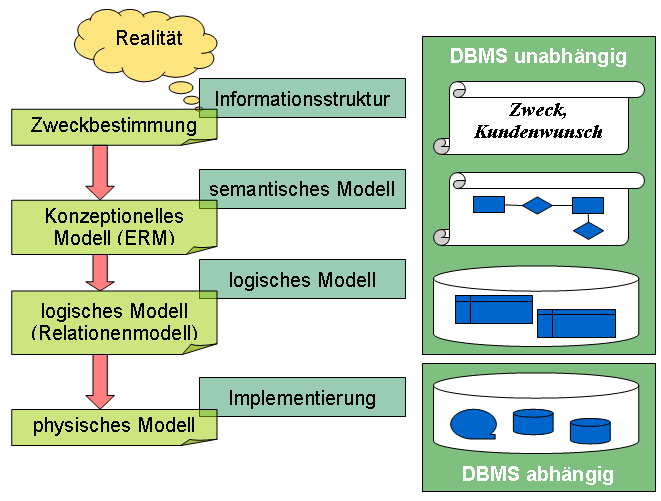
\includegraphics[width=0.7\textwidth]{2jahr_pictures/6lf_oeni_phasen-datenbankentwurf.png}
	\caption{Phasen der Datenbankentwicklung}
	\label{img:6lf_oeni_phasen}
\end{figure}

\subsubsection{Informationsstruktur - Zweckbestimmung}

\subsubsection{Semantisches Modell - ERM}

%%% Anfang: Bild > ERM
\begin{wrapfigure}{l}{0.30\textwidth}
	\begin{center}
		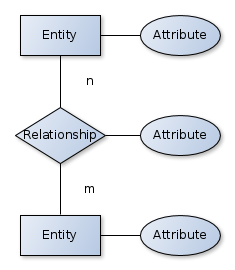
\includegraphics[width=0.30\textwidth]{2jahr_pictures/6lf_oeni_erm-basics.png}
	\end{center}
	\caption{Basics des ERM}
\end{wrapfigure}
%%% Ende: Bild

Bei dem Entity Relationship Model nach Peter Chen gibt es genau definierte Elemente. Dazu gehören drei Formen, das Rechteck, die Elipse und die Raute. Im nebenstehenden Bild ist zu erkennen, welche Form für welches Element steht. 1. Das Rechteck beschreibt Entitätstypen, wobei eine einzelne Entität ähnlich einem Objekt eine Instanz eines Entitätstypes ist. 2. Die Elipse beschreibt Attribute, also Eigenschaften, die ein Entitätstyp haben kann. Beispiele dazu folgen. 3. Die Raute beschreibt die Relationen zwischen verschiedenen Entitätstypen. An den Relationen können drei verschiedene Kardinalitäten die Art der Relation näher bestimmten; a) $1$ zu $1$, b) $1$ zu $n$ und c) $n$ zu $m$. Nur bei $n$ zu $m$ Kardinalitäten können Attribute wie im Bild zu sehen mit eigenen Attributen ausgestattet werden. {\bf Beispiele} für Kardinalitäten. Die $n$ zu $m$ Kardinalität könnte durch ein Attribut wie beispielsweise \ql Dauer\qr\ ergänzt werden.
\begin{itemize}
	\itemsep0em
	\item $1$ zu $1$: \ {\sc Mitarbeiter} hat {\sc Name}
	\item $1$ zu $n$: \ {\sc Mitarbeiter} arbeitet in {\sc Abteilung}
	\item $n$ zu $m$: {\sc Mitarbeiter} arbeitet an {\sc Projekt}
\end{itemize}

\subsubsection{Logisches Modell - Relationenmodell}

Im Anschluss an die Erstellung eines ERM wird das Relationenmodell erstellt. Dabei gilt, dass jeder Entitätstyp einer Tabelle entspricht und jedes Attribut einer Spalte. Die Relationen werden durch Primär- und Fremdschlüssel dargestellt. Bei einer $1$ zu $1$ Relation 

\subsubsection{Physisches Modell - Implementierung}

%%% Ende: Entwurf einer Datenbank
%%%%%%%%%%%%%%%%%%%%%%%%%%%%%%%%%%%%%%%%%%%%%%%%%%%%%%%%%%%%%%%%%%%%%%%%%%%%%%

\subsection{Eine Datenbank entwickeln}
\subsubsection{Normalisierung}

Durch Normalisierung sollen Anomalien und Redundanz in einer Datenbank reduziert werden. Dabei erhöhen sich aber auch die Anforderungen an die Performance. Es werden drei Anomalien unterschieden: (1) Einfüge-Anomalien, (2) Lösch-Anomalien und (3) Änderungs-Anomalie.

(1) Einfüge-Anomalie: neue Daten können nicht angelegt werden, wenn noch nicht alle Informationen bekannt sind.
(2) Lösch-Anomalie: werden Datensätze gelöscht, gehen mehr Informationen verloren, als eigentlich beabsichtigt war.
(3) Änderungs-Anomalie: führen häufig zu Inkonsistenzen

{\bf Erste Normalform}: Die Daten in einer Tabelle müssen atomar (unteilbar) sein und es darf keine Aufzählung (Wiederholungsgruppen) geben. Nach der Übertragung in die erste Normalform (1. NF) kann es notwendig werden, einen neuen (zusammensetzten) Primary Key zu definieren.
{\bf Zweite Normalform}: Die Tabellen muss in der 1. NF sein und jedes Nicht-Schlüsselattribut muss voll funktional vom gesamten Primärschlüssel abhängig sein. Voll funktional bedeutet in diesem Zusammenhang, dass es zum Wert des Primärschlüssels genau einen Wert aus der jeweiligen Spalte des Nicht-Schlüsselattributes gibt.
{\bf Dritte Normalform}: Die tabelle muss sich in der 2. NF befinden und kein Nicht-Schlüsselattribut transitiv vom Primärschlüssel abhängt.
{\bf Boyce-Codd Normalform}: Die Tabelle befindet sich in der 3. NF und keine Teile der Schlüsselkandidaten sind von Nicht-Schlüsselattributen funktional abhängig.

\subsection{Joins - Grundtypen}

Es wird zwischen zwei Grundtypen von Joins unterschieden, OUTER und INNER Joins. OUTER Joins können nochmals in drei Grundtypen unterschieden werden, sodass sich insgesamt vier Grundtypen von Joins ergeben: (1) FULL OUTER, (2) LEFT OUTER, (3) RIGHT OUTER und (4) INNER. Darüber hinaus gibt es noch die beiden Typen NATURAL und SELF JOIN.

Beispiel - A und B
\begin{itemize}
	\item SELECT ... FROM A FULL OUTER JOIN B ON A.id = B.id
	Der Befehl gibt sowohl A als auch B aus.
\end{itemize}

Beispiele - inklusive / exklusive Schnittmenge
\begin{itemize}
	\item SELECT ... FROM A {\it LEFT} OUTER JOIN B ON A.id = B.id
	Der Befehl gibt A {\bf inklusive} der Schnittmenge von A und B aus.
	\item SELECT ... FROM A LEFT OUTER JOIN B ON A.id = B.id WHERE B.id IS NULL
	Der Befehl gibt A {\bf exklusive} der Schnittmenge von A und B aus.
	\item SELECT ... FROM A {\it RIGHT} OUTER JOIN B ON A.id = B.id
	Der Befehl gibt B {\bf inklusive} der Schnittmenge von A und B aus.
	\item SELECT ... FROM A RIGHT OUTER JOIN B ON A.id = B.id WHERE A.id IS NULL
	Der Befehl gibt B {\bf exklusive} der Schnittmenge von A und B aus.
\end{itemize}

Beispiele - Schnittmenge und Komplement
\begin{itemize}
	\item SELECT ... FROM A {\it INNER} JOIN B ON A.id = B.id
	Der Befehl gibt die Schnittmenge von A und B aus.
	\item SELECT ... FROM A FULL OUTER JOIN B ON A.id = B.id WHERE A.id IS NULL OR B.id IS NULL
	Der Befehl gibt das Komplement der Schnittmenge aus - also alles, was sich A und B {\bf nicht} teilen.
\end{itemize}




%\section{Lernfeld 7 - Vernetzte IT-Systeme} % Scheible



\end{document}
